\let\negmedspace\undefined
\let\negthickspace\undefined
\documentclass[journal]{IEEEtran}
\usepackage[a5paper, margin=10mm, onecolumn]{geometry}
%\usepackage{lmodern} % Ensure lmodern is loaded for pdflatex
\usepackage{tfrupee} % Include tfrupee package

\setlength{\headheight}{1cm} % Set the height of the header box
\setlength{\headsep}{0mm}     % Set the distance between the header box and the top of the text

\usepackage{gvv-book}
\usepackage{gvv}
\usepackage{cite}
\usepackage{amsmath,amssymb,amsfonts,amsthm}
\usepackage{algorithmic}
\usepackage{graphicx}
\usepackage{textcomp}
\usepackage{xcolor}
\usepackage{txfonts}
\usepackage{listings}
\usepackage{enumitem}
\usepackage{mathtools}
\usepackage{gensymb}
\usepackage{comment}
\usepackage[breaklinks=true]{hyperref}
\usepackage{tkz-euclide} 
\usepackage{listings}
% \usepackage{gvv}                                        
\def\inputGnumericTable{}                                 
\usepackage[latin1]{inputenc}                                
\usepackage{color}                                            
\usepackage{array}                                            
\usepackage{longtable}                                       
\usepackage{calc}                                             
\usepackage{multirow}                                         
\usepackage{hhline}                                           
\usepackage{ifthen}                                           
\usepackage{lscape}
\begin{document}

\bibliographystyle{IEEEtran}

\title{1.9.12}
\author{EE25BTECH11023 - Venkata Sai}
% \maketitle
% \newpage
% \bigskip
{\let\newpage\relax\maketitle}

\renewcommand{\thefigure}{\theenumi}
\renewcommand{\thetable}{\theenumi}
\setlength{\intextsep}{10pt} % Space between text and floats


\numberwithin{equation}{enumi}
\numberwithin{figure}{enumi}
\renewcommand{\thetable}{\theenumi}


\textbf{Question}:\newline
Find the length of the segment joining \textbf{A}$\brak{-6,7}$ and \textbf{B}$\brak{-1,-5}$. Also, find the
midpoint of AB. 
\\
\textbf{Solution: }
\begin{table}[h!]    
  \centering
  

  \caption{Variables Used}
\end{table}
We use the distance formula between two points $ A\brak{x_1, y_1} $ and $ B\brak{x_2, y_2} $:
\begin{align}
\text{Distance} = \sqrt{\brak{x_2 - x_1}^2 + \brak{y_2 - y_1}^2}
\end{align}

Substitute $ x_1 = -6 $, $ y_1 = 7 $, $ x_2 = -1 $, $ y_2 = -5 $

\begin{align}
\text{Distance} = \sqrt{(-1 - (-6))^2 + (-5 - 7)^2} = \sqrt{(5)^2 + (-12)^2} = \sqrt{25 + 144} = \sqrt{169} = 13
\end{align}

The length of the segment joining $ A $ and $ B $ is 13 sq units. \\

To find midpoint of AB:

Let the required point be P
\begin{align}
AP=\frac{1}{2}AB \implies \frac{AR}{RB}=1\\
\vec{P}=\frac{k(\vec{B})+(\vec{A})}{k+1}=\myvec{x\\y}\\
\end{align}
Here according to problem value of k is 1\\
\begin{align}
P=\frac{B+A}{2}=\frac{\myvec{-6\\7}+\myvec{-1\\-5}}{2}=\frac{\myvec{-7\\2}}{2}\\
\end{align}
\begin{align}
P=\myvec{\frac{-7}{2}\\1}
\end{align}
Hence the coordinates of $\vec{P}$ are $\brak{\frac{-7}{2},1}$
\begin{figure}[h!]
   \centering
   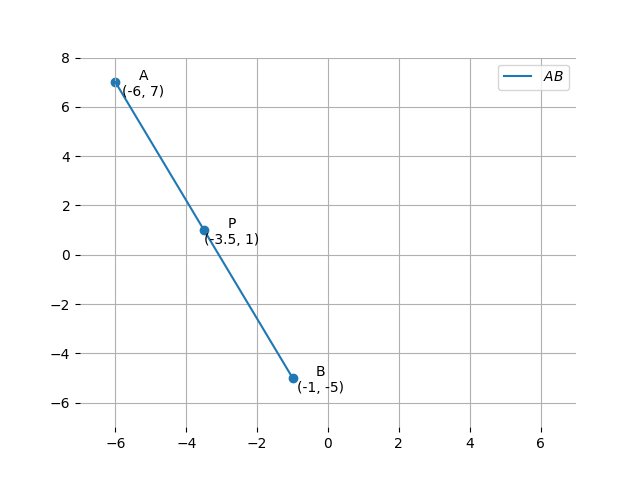
\includegraphics[width=0.7\columnwidth]{figs/fig1.png}
   \caption{Stem Plot of y\brak{n}}
   \label{stemplot}
\end{figure}
\end{document}  